\documentclass[tikz,border=10pt]{standalone}
% Shared look for every TikZ diagram. Load with % Shared look for every TikZ diagram. Load with % Shared look for every TikZ diagram. Load with \input{../../tools/tikz-style.tex}
\usepackage[T1]{fontenc}
\usepackage{lmodern}
\renewcommand{\sfdefault}{lmr}  % diagrams use the same serif as the text
\usetikzlibrary{arrows.meta, positioning, shapes.geometric, calc, fit, backgrounds}
\definecolor{cblue}{HTML}{4C78A8}
\definecolor{corange}{HTML}{F58518}
\definecolor{cgreen}{HTML}{54A24B}
\definecolor{cred}{HTML}{E45756}
\definecolor{cpurple}{HTML}{B279A2}
\definecolor{cgrey}{HTML}{6B6B6B}
\tikzset{
  every picture/.style={font=\sffamily, line width=1.2pt},
  box/.style={draw=#1, fill=#1!12, rounded corners=4pt, align=center, inner sep=7pt, minimum height=1.1cm},
  box/.default=cgrey,
  arrow/.style={-{Stealth[length=3mm]}, draw=cgrey, line width=1.4pt},
  title/.style={font=\sffamily\bfseries\Large},
  note/.style={font=\sffamily\small, text=cgrey, align=center},
}
\AtBeginDocument{\hyphenpenalty=10000 \exhyphenpenalty=10000}

\usepackage[T1]{fontenc}
\usepackage{lmodern}
\renewcommand{\sfdefault}{lmr}  % diagrams use the same serif as the text
\usetikzlibrary{arrows.meta, positioning, shapes.geometric, calc, fit, backgrounds}
\definecolor{cblue}{HTML}{4C78A8}
\definecolor{corange}{HTML}{F58518}
\definecolor{cgreen}{HTML}{54A24B}
\definecolor{cred}{HTML}{E45756}
\definecolor{cpurple}{HTML}{B279A2}
\definecolor{cgrey}{HTML}{6B6B6B}
\tikzset{
  every picture/.style={font=\sffamily, line width=1.2pt},
  box/.style={draw=#1, fill=#1!12, rounded corners=4pt, align=center, inner sep=7pt, minimum height=1.1cm},
  box/.default=cgrey,
  arrow/.style={-{Stealth[length=3mm]}, draw=cgrey, line width=1.4pt},
  title/.style={font=\sffamily\bfseries\Large},
  note/.style={font=\sffamily\small, text=cgrey, align=center},
}
\AtBeginDocument{\hyphenpenalty=10000 \exhyphenpenalty=10000}

\usepackage[T1]{fontenc}
\usepackage{lmodern}
\renewcommand{\sfdefault}{lmr}  % diagrams use the same serif as the text
\usetikzlibrary{arrows.meta, positioning, shapes.geometric, calc, fit, backgrounds}
\definecolor{cblue}{HTML}{4C78A8}
\definecolor{corange}{HTML}{F58518}
\definecolor{cgreen}{HTML}{54A24B}
\definecolor{cred}{HTML}{E45756}
\definecolor{cpurple}{HTML}{B279A2}
\definecolor{cgrey}{HTML}{6B6B6B}
\tikzset{
  every picture/.style={font=\sffamily, line width=1.2pt},
  box/.style={draw=#1, fill=#1!12, rounded corners=4pt, align=center, inner sep=7pt, minimum height=1.1cm},
  box/.default=cgrey,
  arrow/.style={-{Stealth[length=3mm]}, draw=cgrey, line width=1.4pt},
  title/.style={font=\sffamily\bfseries\Large},
  note/.style={font=\sffamily\small, text=cgrey, align=center},
}
\AtBeginDocument{\hyphenpenalty=10000 \exhyphenpenalty=10000}

\begin{document}
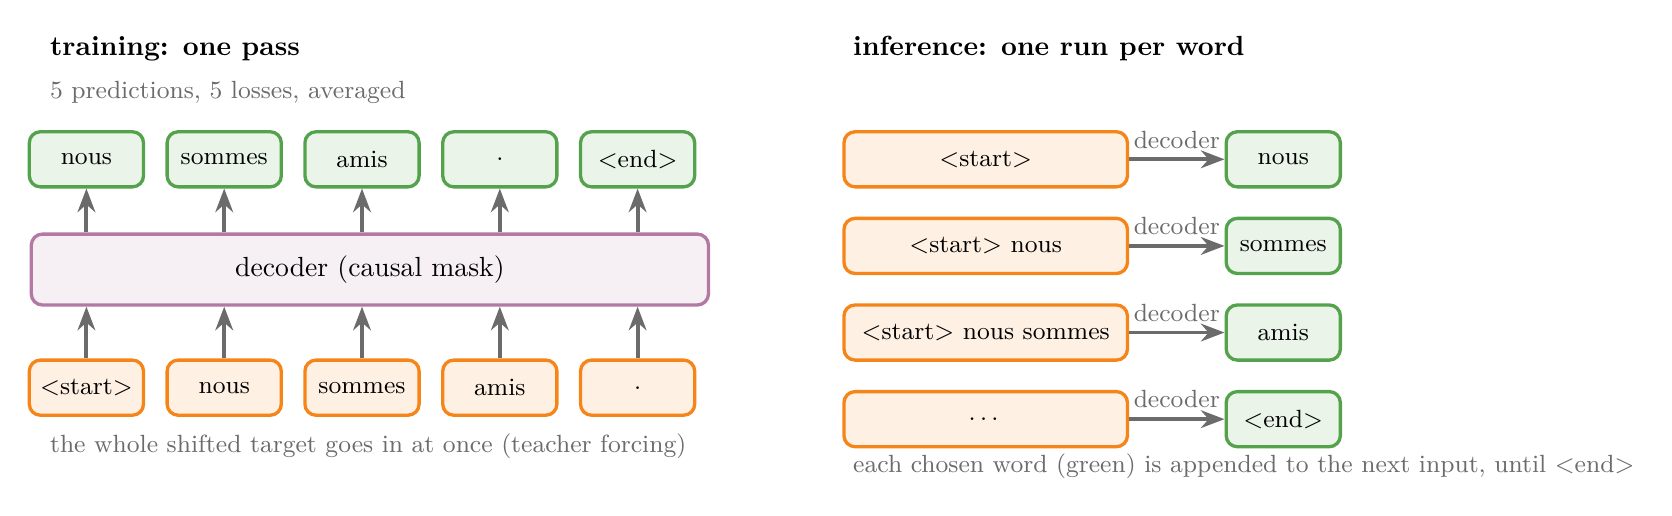
\begin{tikzpicture}[tk/.style={box=#1, minimum width=1.45cm, minimum height=0.7cm, inner sep=2pt, font=\sffamily\small}]
  % training
  \node[font=\sffamily\bfseries, anchor=west] at (-0.6,4.3) {training: one pass};
  \node[box=cpurple, minimum width=8.6cm, minimum height=0.9cm] (dec) at (3.6,1.5) {decoder (causal mask)};
  \foreach \w/\t [count=\k] in {{\textless start\textgreater}/nous, nous/sommes, sommes/amis, amis/., ./{\textless end\textgreater}} {
    \node[tk=corange] (i\k) at (1.75*\k-1.75,0.0) {\w};
    \node[tk=cgreen] (o\k) at (1.75*\k-1.75,2.9) {\t};
    \draw[arrow] (i\k) -- (i\k |- dec.south); \draw[arrow] (o\k |- dec.north) -- (o\k);
  }
  \node[note, anchor=west] at (-0.6,-0.75) {the whole shifted target goes in at once (teacher forcing)};
  \node[note, anchor=west] at (-0.6,3.75) {5 predictions, 5 losses, averaged};
  % inference
  \node[font=\sffamily\bfseries, anchor=west] at (9.6,4.3) {inference: one run per word};
  \foreach \k/\inp/\out in {1/{\textless start\textgreater}/nous, 2/{\textless start\textgreater\ nous}/sommes, 3/{\textless start\textgreater\ nous sommes}/amis, 4/{\dots}/{\textless end\textgreater}} {
    \node[tk=corange, anchor=west, minimum width=3.6cm] (a\k) at (9.6,4.0-1.1*\k) {\inp};
    \node[tk=cgreen] (b\k) at (15.2,4.0-1.1*\k) {\out};
    \draw[arrow] (a\k) -- node[above, note] {decoder} (b\k);
  }
  \node[note, anchor=west] at (9.6,-1.0) {each chosen word (green) is appended to the next input, until \textless end\textgreater};
\end{tikzpicture}
\end{document}
